%-----------------------------------------------------
% Chapter: Introduction
%-----------------------------------------------------
\chapter{Introduction}
\label{chap:intro}
\section{Overview}
Natural language is a constantly evolving system capable of producing infinite numbers of sentences each with their own distinct meaning. The task of inferring meaning from a sentence is one that is seemingly trivial for humans, even from a young age. However, getting machines to derive meaning from textual data has long been a challenge within the field of Artificial Intelligence, specifically the subfield of Natural Language Processing (NLP). Computing numeric representations of words is the first step in bridging the gap between natural language and machines. Previous methods to create such representations include the one-hot encoding method which involves encoding words as word vectors which have as many dimensions as the number of unique words within a corpus. Each dimension in the vector is assigned a zero value except for the dimension representing the word which is assigned a value of 1. For example given a corpus with the following vocabulary 

\begin{center}
\{"Billie", "Jean", "is", "not", "my", "lover"\}
\end{center}

\noindent
and assuming that each word's index represents the dimension of the word, the word vector for "Jean" would be 

\begin{center}
	[0, 1, 0, 0, 0, 0]
\end{center}

\noindent
\newline
The discrete word representations obtained from these types of methods are sparse and suffer from the curse of dimensionality due to the dimensionality of the word vector growing linearly with the size of the vocabulary. Moreover, these representations fail to capture any syntactic and semantic relationships contained within textual data.
 
\noindent
\newline
Recent word representation methods rely on the intuition that word meaning can be inferred from context. Specifically, these methods are based on the distributional hypothesis (\cite{Harris1954}) that states that words which appear in a similar context have similar meanings. Algorithms such as GloVe (\cite{Pennington2014}) and word2vec (\cite{Mikolov2013}) exploit this concept to produce dense continuous word representations which are able to encode syntactic and semantic regularities. These types of distributed representations, first proposed by \cite{Hinton1986},  are also known as \textit{\textbf{word embeddings}} due to the \textit{"embedding"} of words into often low dimensional space.

\noindent
\newline
Often accompanying text corpora are associated covariates such as authorship and publication date, which provide additional metadata about a corpus. Traditional word embedding methods such as GloVe, fail to capture this information and instead rely on individual word embeddings for each subset of data relating to a particular covariate. This approach to creating covariate specific word embeddings has two drawbacks: \textbf{data efficiency}, as performing these methods on subsets is repetitive, and can also yield suboptimal word representations if data is scarce for a particular subset, and decreased \textbf{interpretability}, due to the random initialisation of word embeddings, which even when created with the same random seed, produce representations relative to the the structure of the text. 

\noindent
\newline
CoVeR (\cite{Tian2018}), a novel tensor decomposition method for learning covariate specific word embeddings, is an extension of the GloVe algorithm which aims to efficiently encode covariate information within learned embeddings whilst increasing interpretability. The goal of this project, is to explore the effectiveness of CoVeR generated word embeddings as well as its potential application within a prototype software aimed at songwriters. 

\noindent
\newline
The motivation behind using CoVeR is two-fold. Firstly, its efficient use of data is beneficial when data isn't readily available, which, in the case of this project and song lyrics, is true (discussed more in \autoref{chap:prof_con}) and its increased interpretability compared to traditional methods which allows for greater analysis. The next section briefly contextualises the project, highlighting common issues songwriters face during the writing process.

\section{The Songwriters Dilemma}
Songwriting is an integral part of the song making process which often draws upon past events and experiences. Structure and content both contribute heavily towards the success of a song; with the latter being a key factor on the extent to which a song resonates with a listener. A problem commonly faced by songwriters is that of word choice, through which they can express their ideas clearly and concisely.

\noindent
\newline
Skilled writers are commonly attributed with having vast vocabulary ranges. For adults, the average vocabulary size ranges between 15,000 - 23,000 words (\cite{McCrum2011}). Examining his works alone, Shakespeare is said to have had an approximate vocabulary range of 30,000 - 65,000 words\footnote{https://kottke.org/10/04/how-many-words-did-shakespeare-know} \footnote{This range is most likely skewed as variant forms of words are included as singular counts}. Nonetheless, a skilled songwriters ability to write impactful lyrics is not down to vocabulary size alone, but effective word choice.
 
\noindent
\newline
As shown in a study examining vocabulary range within Hip Hop\footnote{https://pudding.cool/projects/vocabulary/index.html}, which recently surpassed Rock as the most popular genre in the United States\footnote{https://www.nielsen.com/us/en/insights/reports/2018/2017-music-us-year-end-report.html}, more is not always better. The study examines the unique word count of 150 famous Hip Hop artists across their first 35,000 words used in lyrics. Aesop Rock, ranked 1st on the list, recorded a count of 7,392 unique words across his first 35,000 words. In contrast, rappers Drake and Future, who ranked 130th and 131st respectively, had an average unique word count of 3,334 words used across their first 35,000 words; a 55\% decrease from Aesop Rocks count. 
\begin{figure}[h]	
	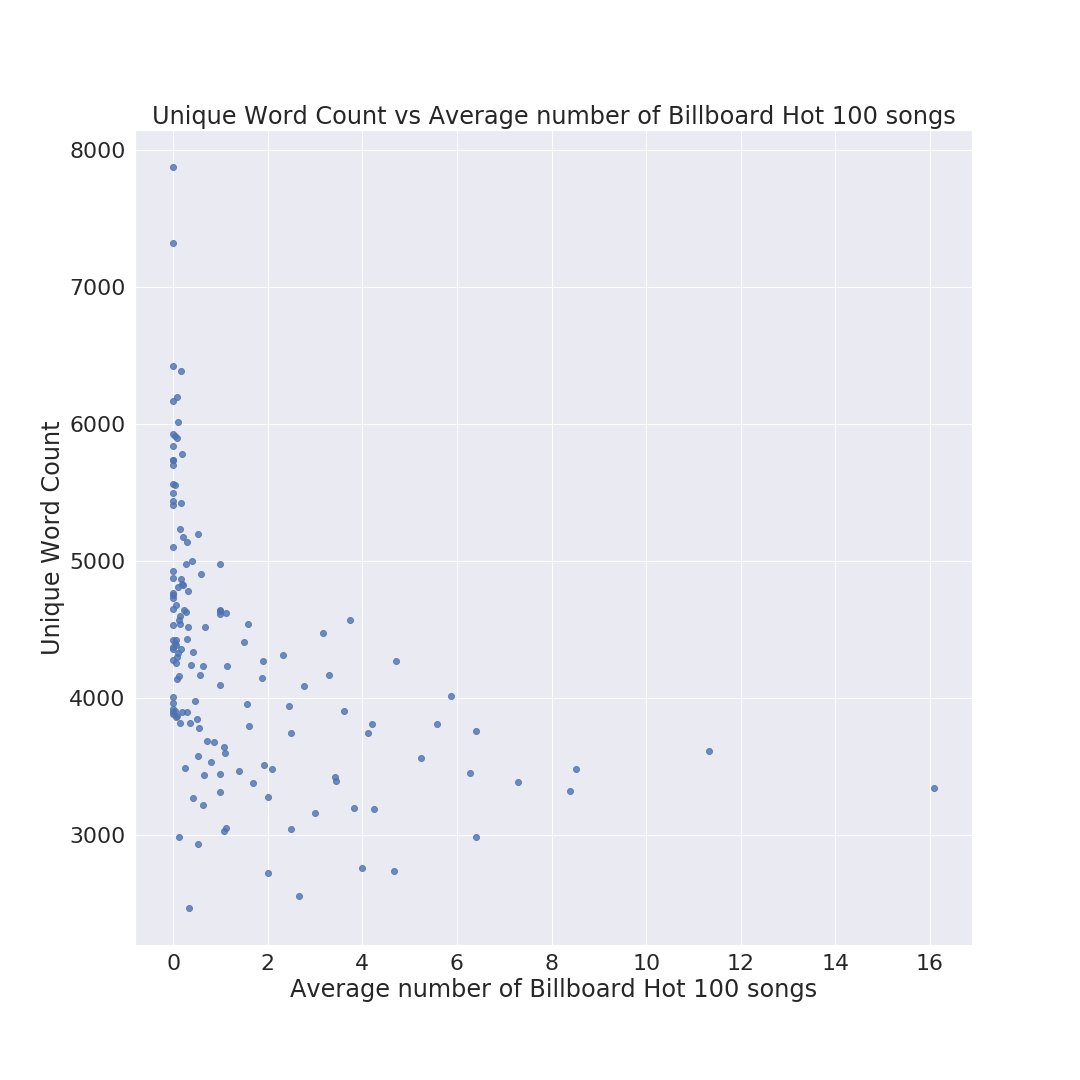
\includegraphics[width=13cm, height=13cm]{./figures/fig1}
	\centering
	\caption[Average Number of Billboard Hot 100 songs vs Unique Word Count]{Average number of Billboard Hot 100 songs during artist activity, compared to unique word count across an artists first 35,000 words.}
	\label{fig:fig1}
\end{figure}

\noindent
\newline
To validate the earlier claim that vocabulary range is not indicative of a songwriters ability to write impactful lyrics, the unique word count per artist was compared against the average number of Billboard 100\footnote{https://www.billboard.com/charts/hot-100} \footnote{The Billboard Hot 100 is a ranking chart of the 100 most played songs in the United States based on sales, radio play and online streaming.} songs an artist had obtained across their career (seen in \autoref{fig:fig1}). Pearson's Correlation Coefficient, which is used to measure the linear relationship between two variables, was applied to both unique word count and average number of Billboard 100 songs. This resulted in a correlation coefficient of - 0.42, indicating a weak inverse correlation between the pairs of data. This value supports the earlier claim that vocabulary range is not indicative of a songwriters ability.

\noindent
\newline
Common methods used to improve songwriting competency include group writing and vocabulary expansion. More recently, software solutions such as MasterWriter\footnote{https://masterwriter.com/5} have been used to consolidate previous methods. An inherent drawback with applications such as MasterWriter is the static nature of features such as fixed word dictionaries and thesauruses. Consequently, these applications fail to capture the ever changing nature of language.

\noindent
\newline
After the completion of song lyrics, another task in the song making process, if not already completed, is song production. For experienced songwriters, production choice might be a routine decision due to them having an established production style. On the other hand, for newer songwriters or songwriter's wishing to experiment with a new sound, this choice may not be a trivial one, especially with the constant increase in the popularity and existence of genres and subgenres, which come with their respective production styles. As shown in \autoref{fig:fig11}, the distribution of music genres listened to has spread over time, even more so, the increase of distinctive sub genres within these genres.

\begin{figure}[h]	
	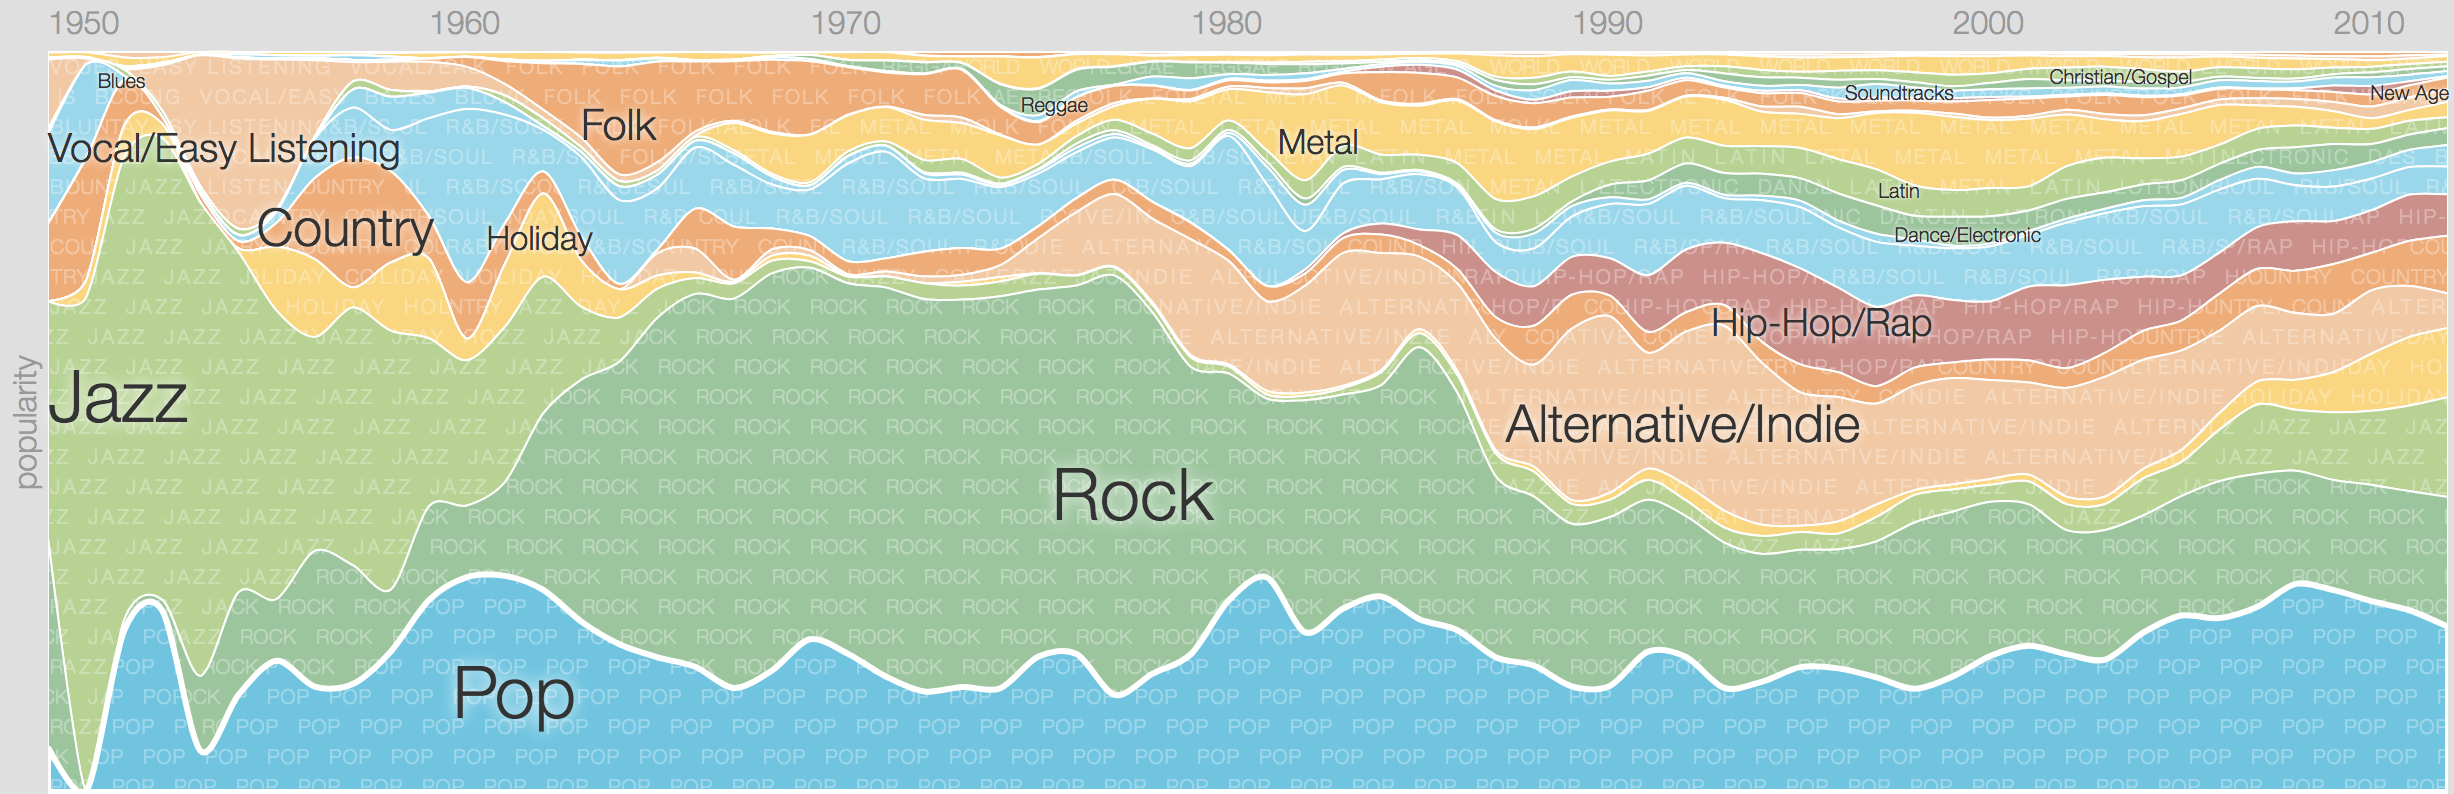
\includegraphics[width=14cm, height=5cm]{./figures/fig11}
	\centering
	\caption[Distribution of music genres listened to from 1950]{Distribution of music genres listened from 1950, based on the music library of Google Play Users.}
	\footnote{hello}
	\label{fig:fig11}
\end{figure}

\section{Aims and Objectives}
\noindent
\newline
As previously stated, the goal of this project is to explore effectiveness of CoVeR as well as its potential usage in a software application. Specifically this takes the form of a prototype software solution to help reduce common problems faced by songwriters, namely:

\begin{enumerate}
	\item Word Choice 
	\item Lyric classification
\end{enumerate}

\noindent
\newline
The tasks of predicting the next word in a song and lyric classification can viewed as abstracted forms of two common NLP tasks: \textit{Language Modelling} and \textit{Text Classification}, which are two active research areas in NLP that have benefited greatly from word embeddings. The usage of these word embeddings has helped improve accuracy in tasks such as Machine Translation (\cite{Qi2018}) and Document Classification (\cite{Manning2008}). State of the art results in both areas have also utilised recurrent neural networks (RNN), (discussed in \autoref{chap:background}) which employ word embeddings within the input layer to the network.

\noindent
\newline
With this in mind, a prototype solution, SONGIFAI is proposed. SONGIFAI provides two main features namely lyric assistance through predictive text and a word suggestion feature, as well as genre classification for a given song lyrics. The covariates explored in this project are the following music genres: \textit{Pop}, \textit{Rock} and \textit{Hip Hop}. 

\noindent
\newline
As stated before, RNN's have been used successfully in both language modelling and text classification tasks. The specific variant of the recurrent neural network which has been successfully utilised in these tasks is the Long Short-Term Memory (LSTM) network (discussed in \autoref{chap:background}). This network architecture is used for both the language model and text classifier which are applied to the word prediction and lyric classification features respectively. The word suggestion feature utilises the covariate specific embeddings themselves. A high level system architecture of the prototype can be seen in \autoref{fig:fig7}5
\begin{figure}[h]	
	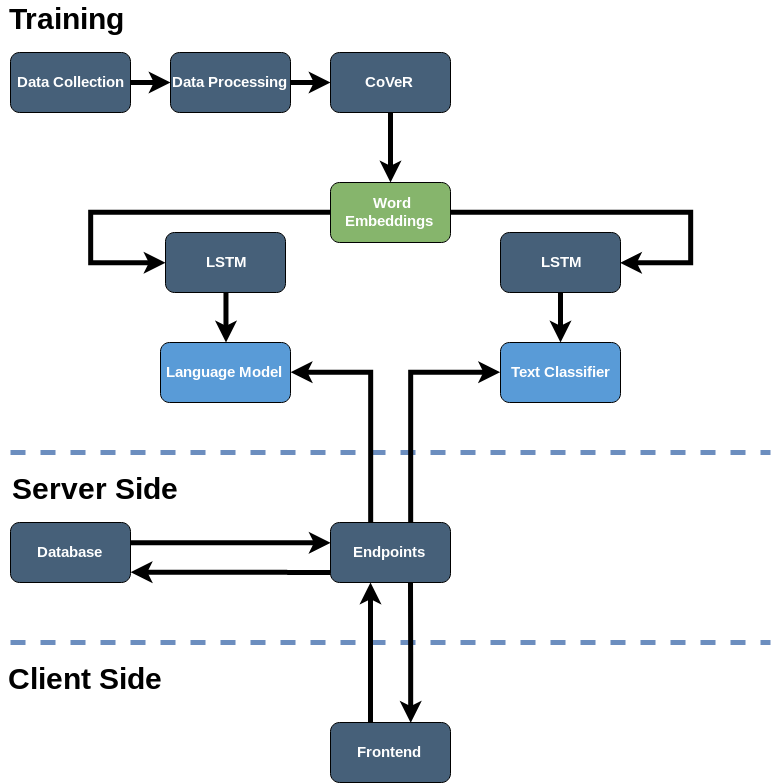
\includegraphics[width=15cm, height=16cm]{./figures/fig7}
	\centering
	\caption[SONGIFAI: High Level Architecture]{From a high level, the system can be split into three sections: \textbf{Training}, where models are created. \textbf{Server Side}, a Python based API used to interface with the trained models.\textbf{Client Side} a user interface built using JavaScript}.
	\label{fig:fig7}
\end{figure}
